\subsubsection{Routing information}
\label{sec:sphinx:routinginformation}

Each node on the path needs to decide whether it is destined to be the receiver of the message and if not, to whom it is supposed to forward the packet. To achieve the privacy properties, each node must only know its direct predecessor and successor along the chosen path. More precisely, the node must not be able to determine \textit{if} and \textit{where} the next downstream node is going to forward the packet to. This is achieved by blinding that information such that it is visible to only that node who needs it.

To ensure that the header has not been tampered while transfered through the network and processed by nodes along the path, routing information contains also an integrity tag to check for modifications before processing the packet. Hence, the routing information for each node by $(y_i, \gamma_i)$ where $y_i$ denotes the public key and $\gamma_i$ the integrity tag for the next downstream node. See section \ref{sec:sphinx:integrity} for more details on the utilized integrity scheme.

\paragraph{Adresses}

Nodes in the network are distinguished by the ECDSA public keys, hence the header includes the public key of the next downstream node and a distinguished byte sequence $END$ to notify the last node on the path that it is the final recipient.

ECDSA public keys are given by tuple of two 32-byte field elements $(x,y)$, upon which it is sufficient to solely store the first component $x$ and the sign of $y$, resulting in a \textsf{compressed} elliptic curve point \textsf{0x02}\textless\textsf{x}\textgreater for positive $y$ and \textsf{0x03}\textless\textsf{x}\textgreater. The sequence $END$ is given as \textsf{0x04} such that the last node can ignore all subsequent bytes if $END$ is present.

\paragraph{Blinding}

The header uses multiple blindings and their aggregations to make certain sections of the header visible to only a single node. Blindings are generated by a pseudorandomness generator (PRG), see appendix \ref{appendix:prg} for a detailed description of the utilized PRG.

As a result of the Diffie-Helman key exchange done in section \ref{appendix:keyderivation}, each node along the path is able to derive a shared secret $s_i$ with the creator of the packet and is therefore able to derive a sub-key $s_i^{bl}$. Both, creator of the packet and each node $n_i$ along the path use $s_i^{bl}$ as a seed for the PRG, yielding $blinding_i$.

The routing information for each node $n_i$ is blinded by XORing the content with $blinding_i$ as well as the blindings $blinding_0, \dots , blinding_{i-1}$ of all previous hops. Each node that receives the packet, removes their own blinding from the header and is thus able extract the routing information destined for them. By removing the blinding from the header, it allows the next downstream node to extract their routing information since it is now only blinded by their blinding.

\begin{figure}[H]
    \centering
    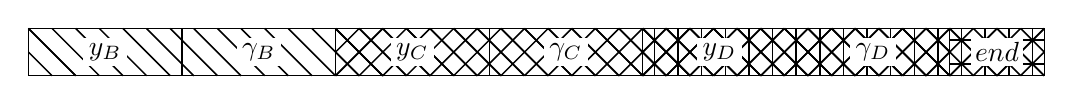
\begin{tikzpicture}
        \def\one{0.6}
        \def\scale{0.9}
        \def\nodeWidth{1.95}
        \def\endWidth{1.2}
        \def\width{3*2*\nodeWidth+\endWidth}
        \foreach \i\name in{0/B,1/C,2/D,3/Z} {
                \begin{scope}[shift={(\i*\nodeWidth*2,0)}]
                    \ifnum\i=0
                        \def\a{11.7}
                        \def\diff{11.1}
                    \fi

                    \ifnum\i=1
                        \def\a{7.8}
                        \def\diff{7.2}
                    \fi

                    \ifnum\i=2
                        \def\a{3.9}
                        \def\diff{3.3}

                    \fi

                    \ifnum\i=3
                        \def\a{\endWidth}
                        \def\diff{0.6}
                    \fi


                    \def\b{0.6}
                    \def\lw{0.2}

                    \foreach \x [count=\i] in{0,0.3,0.6,...,\b}{
                            \draw [line width=\lw mm](\x,0)--(0,\x) (\a-\b+\x,\b)--(\a,\x);
                        }
                    \foreach \x [count=\i] in{0,0.3,0.6,...,\diff}{
                            \draw [line width=\lw mm](\x+\b,0)--(\x,\b);
                        }

                    \ifnum\i>0
                        \foreach \x [count=\i] in{0,0.3,0.6,...,\b}{
                                \draw [line width=\lw mm](0,\x)--(\b-\x,\b) (\a-\b+\x,0)--(\a,\b-\x);
                            }
                        \foreach \x [count=\i] in{0,0.3,0.6,...,\diff}{
                                \draw [line width=\lw mm](\x,0)--(\b+\x,\b);
                            }
                    \fi

                    \ifnum\i>1
                        \foreach \x [count=\i] in{0.15,0.45,...,\a}{
                                \draw [line width=\lw mm](\x,0)--(\x,\b);
                            }
                    \fi

                    \ifnum\i>2
                        \foreach \x [count=\i] in{0.15,0.45,...,\b}{
                                \draw [line width=\lw mm](0,\x)--(\a,\x);
                            }
                    \fi
                \end{scope}
                \ifnum\i<3
                    \draw [color=white] (\i*2*\nodeWidth,0) rectangle (\i*2*\nodeWidth+\nodeWidth,\one) node [midway,color=black,fill=white,inner sep=2pt] {$y_{\name}$};
                    \draw (\i*2*\nodeWidth,0) -- (\i*2*\nodeWidth,\one);
                    \draw [color=white] (\i*2*\nodeWidth+\nodeWidth,0) rectangle (\i*2*\nodeWidth+2*\nodeWidth,\one) node [midway,color=black,fill=white,inner sep=2pt] {$\gamma_{\name}$};
                    \draw (\i*2*\nodeWidth+\nodeWidth,0) -- (\i*2*\nodeWidth+\nodeWidth,\one);
                \else
                    \draw [color=white] (\i*2*\nodeWidth,0) rectangle (\i*2*\nodeWidth+\endWidth,\one) node [midway,color=black,fill=white,inner sep=1.5pt] {$end$};
                    \draw (\i*2*\nodeWidth,0) -- (\i*2*\nodeWidth,\one);
                \fi
            }

        \draw (0,0) rectangle (\width,\one);
    \end{tikzpicture}
    \caption{Blinded routing information sent to first relayer $B$.}
\end{figure}

\paragraph{Filler}



such that $y_Z$ is the destination's public key in compressed form (since this is only the $x$-coordinate, it is 33 bytes instead of 64) and $|y_Z|$ is its length. $\rho$ is a pseudorandom generator (PRG) and $h_{\rho}$ is the hash function used to key $\rho$.
$v\leq r$ is the length of the path traversed by the packet, where $|y_Z| \leq (2(r - v) + 2)$. $\phi$ is a filler string such that
\begin{align}
    \phi_i & =\{ \phi_{i-1}\|0_{2\kappa}\}\oplus \rho(h_{\rho}(s_{i-1}))_{[ \,(2(r-i)+3)\kappa..(2r+3)\kappa-1\,]}
\end{align}
where $\phi_0=\epsilon$ is an empty string. $\phi_i$ is generated using the shared secret $s_{i-1}$ and used to ensure the header packets remain constant in size as layers of encryption are added or removed. Upon receiving a packet, the processing node extracts the information destined for it from the route information and the per-hop payload. The extraction is performed by deobfuscating and left-shifting the field. Ordinarily, this would make the field shorter at each hop, allowing an attacker to deduce the route length. For this reason, the field is pre-padded before forwarding. Since the padding is part of the HMAC, the origin node will have to pre-generate an identical padding (to that generated at each hop) in order to compute the HMACs correctly for each hop.

\begin{figure}[H]
    \centering
    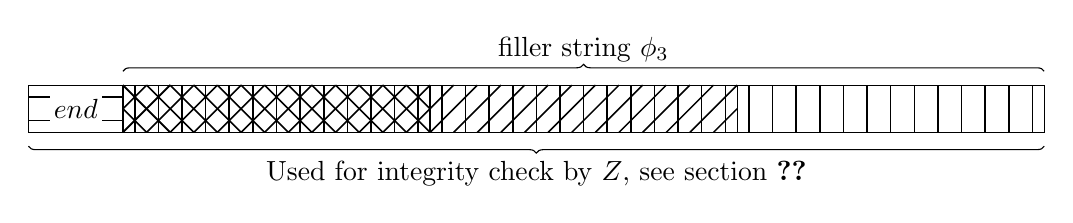
\begin{tikzpicture}
        \def\one{0.6}
        \def\scale{0.9}
        \def\nodeWidth{1.95}
        \def\endWidth{1.2}
        \def\width{3*2*\nodeWidth+\endWidth}
        \foreach \i\name in{0/B,1/C,2/D,3/Z} {
                \ifnum\i=3
                    \def\a{11.7}
                    \def\diff{11.1}
                \fi

                \ifnum\i=2
                    \def\a{7.8}
                    \def\diff{7.2}
                \fi

                \ifnum\i=1
                    \def\a{3.9}
                    \def\diff{3.3}

                \fi

                \ifnum\i=0
                    \def\a{\endWidth}
                    \def\diff{0.6}
                \fi


                \def\b{0.6}
                \def\lw{0.2}

                \begin{scope}[shift={(\endWidth,0)}]
                    \ifnum\i=1
                        \foreach \x [count=\i] in{0,0.3,0.6,...,\b}{
                                \draw [line width=\lw mm](\x,0)--(0,\x) (\a-\b+\x,\b)--(\a,\x);
                            }
                        \foreach \x [count=\i] in{0,0.3,0.6,...,\diff}{
                                \draw [line width=\lw mm](\x+\b,0)--(\x,\b);
                            }
                    \fi

                    \ifnum\i=2
                        \foreach \x [count=\i] in{0,0.3,0.6,...,\b}{
                                \draw [line width=\lw mm](0,\x)--(\b-\x,\b) (\a-\b+\x,0)--(\a,\b-\x);
                            }
                        \foreach \x [count=\i] in{0,0.3,0.6,...,\diff}{
                                \draw [line width=\lw mm](\x,0)--(\b+\x,\b);
                            }
                    \fi

                    \ifnum\i=3
                        \foreach \x [count=\i] in{0.15,0.45,...,\a}{
                                \draw [line width=\lw mm](\x,0)--(\x,\b);
                            }
                    \fi
                \end{scope}

                \ifnum\i=0
                    \foreach \x [count=\i] in{0.15,0.45,...,\b}{
                            \draw [line width=\lw mm](0,\x)--(\a,\x);
                        }
                \fi
                \ifnum\i>0
                    % \draw [color=white] (\i*2*\nodeWidth,0) rectangle (\i*2*\nodeWidth+\nodeWidth,\one) node [midway,color=black,fill=white,inner sep=2pt] {$y_{\name}$};
                    \draw (\i*2*\nodeWidth+\endWidth,0) -- (\i*2*\nodeWidth+\endWidth,\one);
                    % \draw [color=white] (\i*2*\nodeWidth+\nodeWidth,0) rectangle (\i*2*\nodeWidth+2*\nodeWidth,\one) node [midway,color=black,fill=white,inner sep=2pt] {$\gamma_{\name}$};
                    % \draw (\i*2*\nodeWidth+\nodeWidth,0) -- (\i*2*\nodeWidth+\nodeWidth,\one);
                \else
                    \draw [color=white] (\i*2*\nodeWidth,0) rectangle (\i*2*\nodeWidth+\endWidth,\one) node [midway,color=black,fill=white,inner sep=1.5pt] {$end$};
                    \draw (\endWidth,0) -- (\endWidth,\one);
                \fi
            }

        \draw (0,0) rectangle (\width,\one);
        \draw[decoration={brace,raise=5pt},decorate] (\endWidth,\one) -- node[above=5pt] {filler string $\phi_3$} (\width,\one);
        \draw[decoration={brace,mirror,raise=5pt},decorate] (0,0) -- node[below=7pt] {Used for integrity check by $Z$, see section \ref{sec:sphinx:integrity}} (\width,0);


    \end{tikzpicture}
    \caption{Transformed header as seen by $Z$}
\end{figure}

$\beta_i$ is computed as the concatenation of $y_Z$ and a sequence of padding which is then encrypted by XORing with the output of a PRG seeded with shared key $s_{v-1}$ of node $v-1$. The result is finally concatenated with $\phi$ to ensure the header packets remain constant in size.

In the original Sphinx paper, $y_Z$ is concatenated with an identifier $I$ and $0$ padding sequence, where $I$ is used for SURBs (single-use reply blocks) such that $I \in \{0, 1\}^\kappa$. We do not use $I$ since HOPR does not currently employ SURBs. We do, however, include $hint$ and $challenge$ values in $\beta$, defined in the \lcnameref{sec:proofofrelay} section. These values are not included in the original Sphinx paper but are needed for the HOPR protocol. Since $A$ has a shared secret with each of the nodes along the path, it is able to derive blindings for each of them. Each node along the path receives an authentication tag $\gamma_i$ in the form of a message authentication code (MAC), which is encoded in the header.

Padding is added at each mix stage in order to keep the length of the message invariant at each hop.

The mix header is constructed as follows:
\begin{align}
    M_i & =(\alpha_i,\beta_i,\gamma_i)
\end{align}

$A$ sends the mix header $M_0$ to $B$. Once $B$ receives the packet, it derives the shared key $s_0$ by computing

$$s_0=(\alpha_0)^b=(g^x)^b=(g^b)^x=y^x_B$$

and removes its blindings. Here $b$ is the private key of node B. This allows $B$ to unblind the routing info that tells $B$ the public key of the next downstream node, $C$. The process happens in the same fashion for all further downstream nodes after $B$.

